\newpage
\section{Descrizione design pattern}
\subsection{Introduzione}
I \glo{Design pattern}{design pattern} semplificano l'attività di progettazione, favorendo il riutilizzo del codice e rendendo l'architettura più manutenibile. I design pattern vengono definiti come soluzioni progettuali generali a problemi ricorrenti. Si tratta di una descrizione o dei modelli logici da applicare per la risoluzione di problemi che possono presentarsi durante la \glo{Fase}{fase} di progettazione. Esistono diversi design pattern e vengono suddivisi in base al problema da risolvere:
\begin{itemize}
	\item \textbf{pattern creazionali}: nascondono i costruttori delle classi e espongono dei metodi al loro posto. In questo modo si possono utilizzare oggetti senza sapere come sono implementati;
	\item \textbf{pattern comportamentali}: forniscono soluzione alle più comuni tipologie di interazione tra gli oggetti;
	\item \textbf{pattern architetturali}: operano ad un livello più elevato rispetto ad altri design pattern, ed esprimono schemi di base per impostare l'organizzazione strutturale di un sistema software. In questi schemi si descrivono sottosistemi predefiniti, i ruoli che essi assumono e le relazioni reciproche;
	\item \textbf{pattern strutturali}: consentono di riutilizzare degli oggetti esistenti fornendo agli utilizzatori un'interfaccia più adatta alle loro esigenze.
\end{itemize}
Sono stati utilizzati i seguenti design pattern:
\begin{itemize}
	\item Abstract Factory (creazionale);
	\item Builder (creazionale);
	\item Factory Method (creazionale);
	\item Facade (strutturale);
	\item Redux (architetturale).
\end{itemize}

Di seguito verranno mostrati i design pattern utilizzati e come vengono contestualizzati nel progetto \progetto{}. I diagrammi delle classi mostrati in queste comparazioni sono parziali e a scopo illustrativo. Per la loro visualizzazione completa si rimanda alla sezione \ref{componenti}.

\newpage
\subsection{Pattern Creazionali}
\subsubsection{Abstract Factory Method}
\paragraph{Descrizione}
Lo scopo dell'Abstract Factory Method è fornire un interfaccia per creare famiglie di oggetti correlati o dipendenti senza specificare quali siano le loro classi concrete.
In questo modo si permette che un sistema sia indipendente dall'implementazione degli oggetti concreti e che il client, attraverso l'interfaccia, utilizzi diverse famiglie di prodotti.
\\Questo pattern è utile quando:
\begin{itemize}
	\item 	si vuole un sistema indipendente da come gli oggetti vengono creati, composti e rappresentati;
	\item 	si vuole permettere la configurazione del sistema come scelta tra diverse famiglie di prodotti;
	\item 	si vuole fornire una \glo{Libreria}{libreria} di classi mostrando solo le interfacce e nascondendo le implementazioni.
\end{itemize}
\paragraph{Contestualizzazione}
Il pattern Abstract Factory Method viene utilizzato nel \glo{Package}{package} \texttt{ViewPkg} per la creazione dell'oggetto di tipo \texttt{Sidebar}.
In particolare è stato introdotto un livello in più di astrazione rispetto al design pattern comunemente conosciuto, per legare tra loro le tipologie di \texttt{Sidebar} creabili.
\texttt{AbstractSideBarFactory} e le sue cinque sottoclassi astratte:
\begin{itemize}
	\item \texttt{AbstractAssetSidebarFactory};
	 \item \texttt{AbstractNodeSidebarFactory};
	 \item \texttt{AbstractEdgeSidebarFactory};
	 \item \texttt{AbstractScenarioSidebarFactory};
	 \item \texttt{AbstractAnalysisSidebarFactory}.
\end{itemize}
dichiarano soltanto un'interfaccia per la creazione di sidebar, mentre la responsabilità della creazione effettiva delle istanze è delle sottoclassi concrete. È stato quindi definito un metodo di factory per ogni Sidebar. Le factory concrete specificano poi i propri prodotti ridefinendo per ciascuno di essi il metodo factory.
	\begin{figure}[H]
		\label{builder_compara}
		\centering
		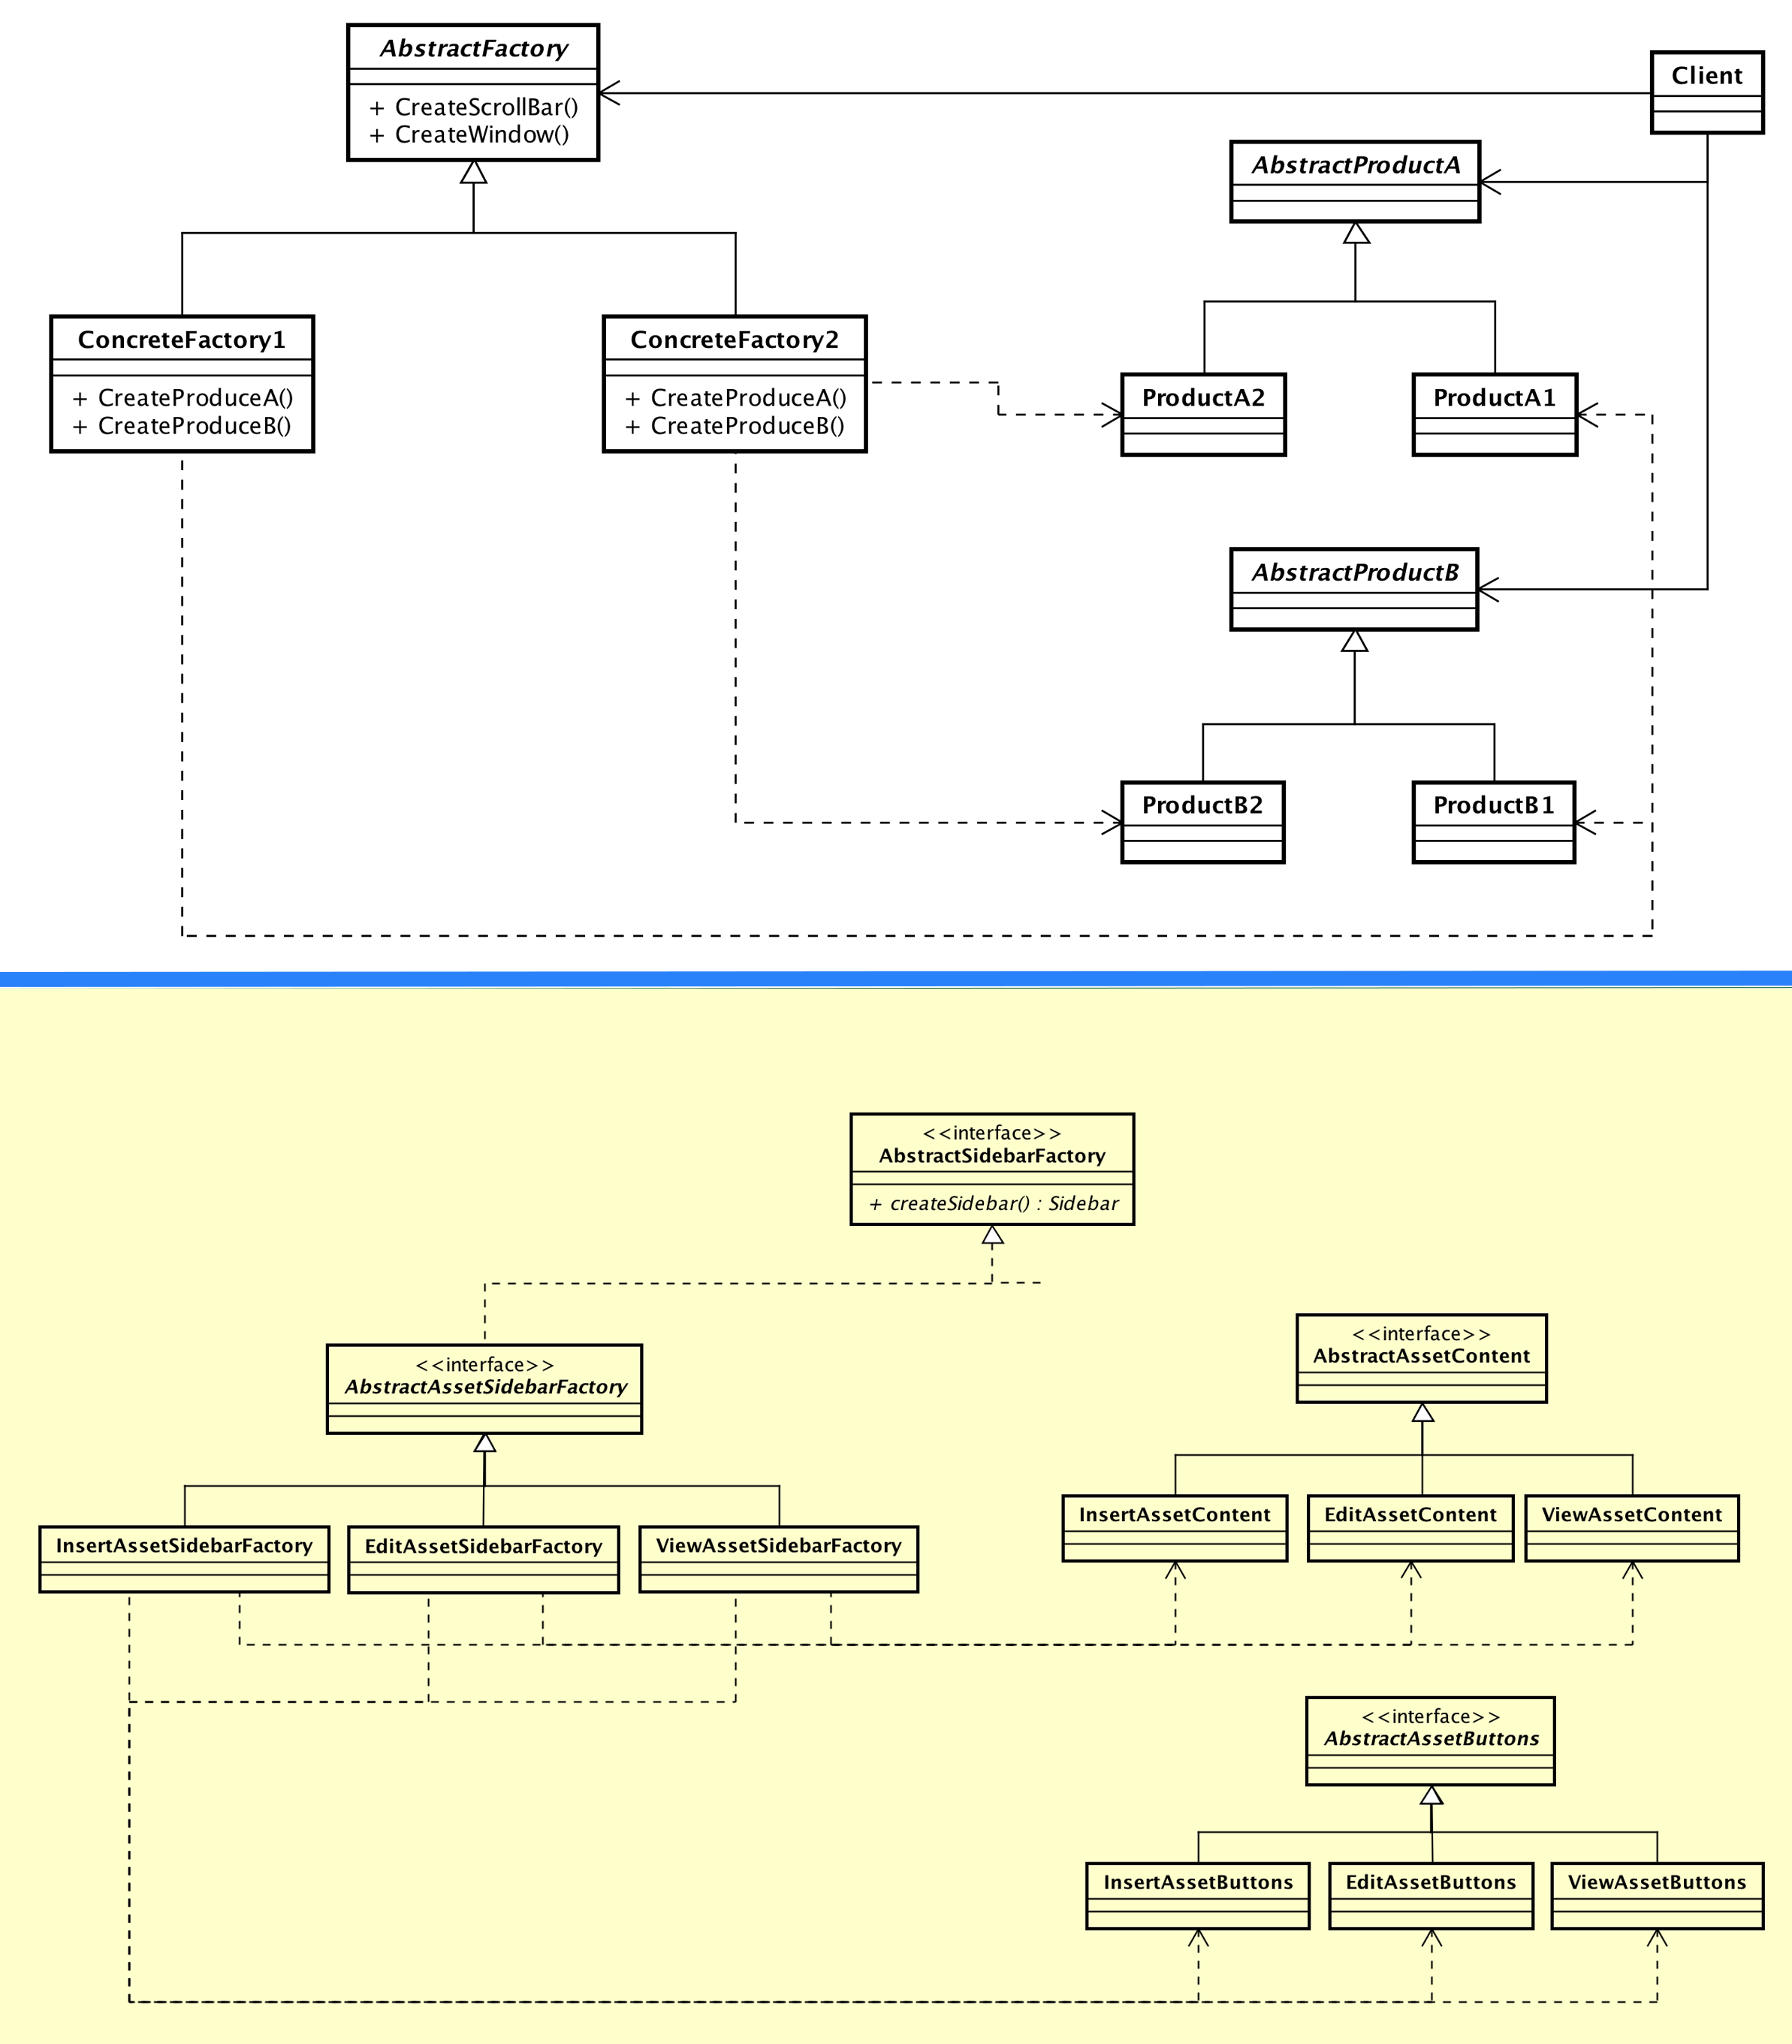
\includegraphics[width=\textwidth]{img/absComparati.png}
		\caption{Abstract Factory ed estratto della sua contestualizzazione in \progetto}
	\end{figure}

\newpage
\subsubsection{Builder}
\paragraph{Descrizione}
Il Builder pattern, permette di separare la costruzione di un oggetto complesso dalla sua rappresentazione sicché il processo di costruzione stesso possa creare diverse rappresentazioni.
L'algoritmo per la creazione di un oggetto complesso è indipendente da come le varie parti vengono assemblate e così la separata classe builder si focalizza sulla corretta costruzione di un'istanza mentre la classe originale si concentra sul funzionamento degli oggetti. Ciò è particolarmente utile quando si vuole assicurare che un oggetto sia valido prima di istanziarlo, e che la logica di controllo non appaia nei costruttori degli oggetti. Un builder permette anche di costruire un oggetto passo-passo, cosa che si può verificare quando si fa il parsing di un testo o si ottengono i parametri da un'interfaccia interattiva.
\paragraph{Contestualizzazione}
Questo pattern viene utilizzato nel package  \texttt{ViewPkg} per la creazione di un oggetto di tipo  \texttt{DeGeOPView}.
\\E' stata creata l'interfaccia \texttt{DeGeOPViewBuilder} che definisce le operazioni che agiscono sull'elemento \texttt{DeGeOPView} che il \texttt{Director} chiederà di creare. Il  \texttt{ConcreteDeGeOPViewBuilder} sovrascriverà tali operazioni, incapsulando il modo di costruire e rappresentare l'oggetto \texttt{DeGeOPView}.
	\begin{figure}[H]
		\label{builder_compara}
		\centering
		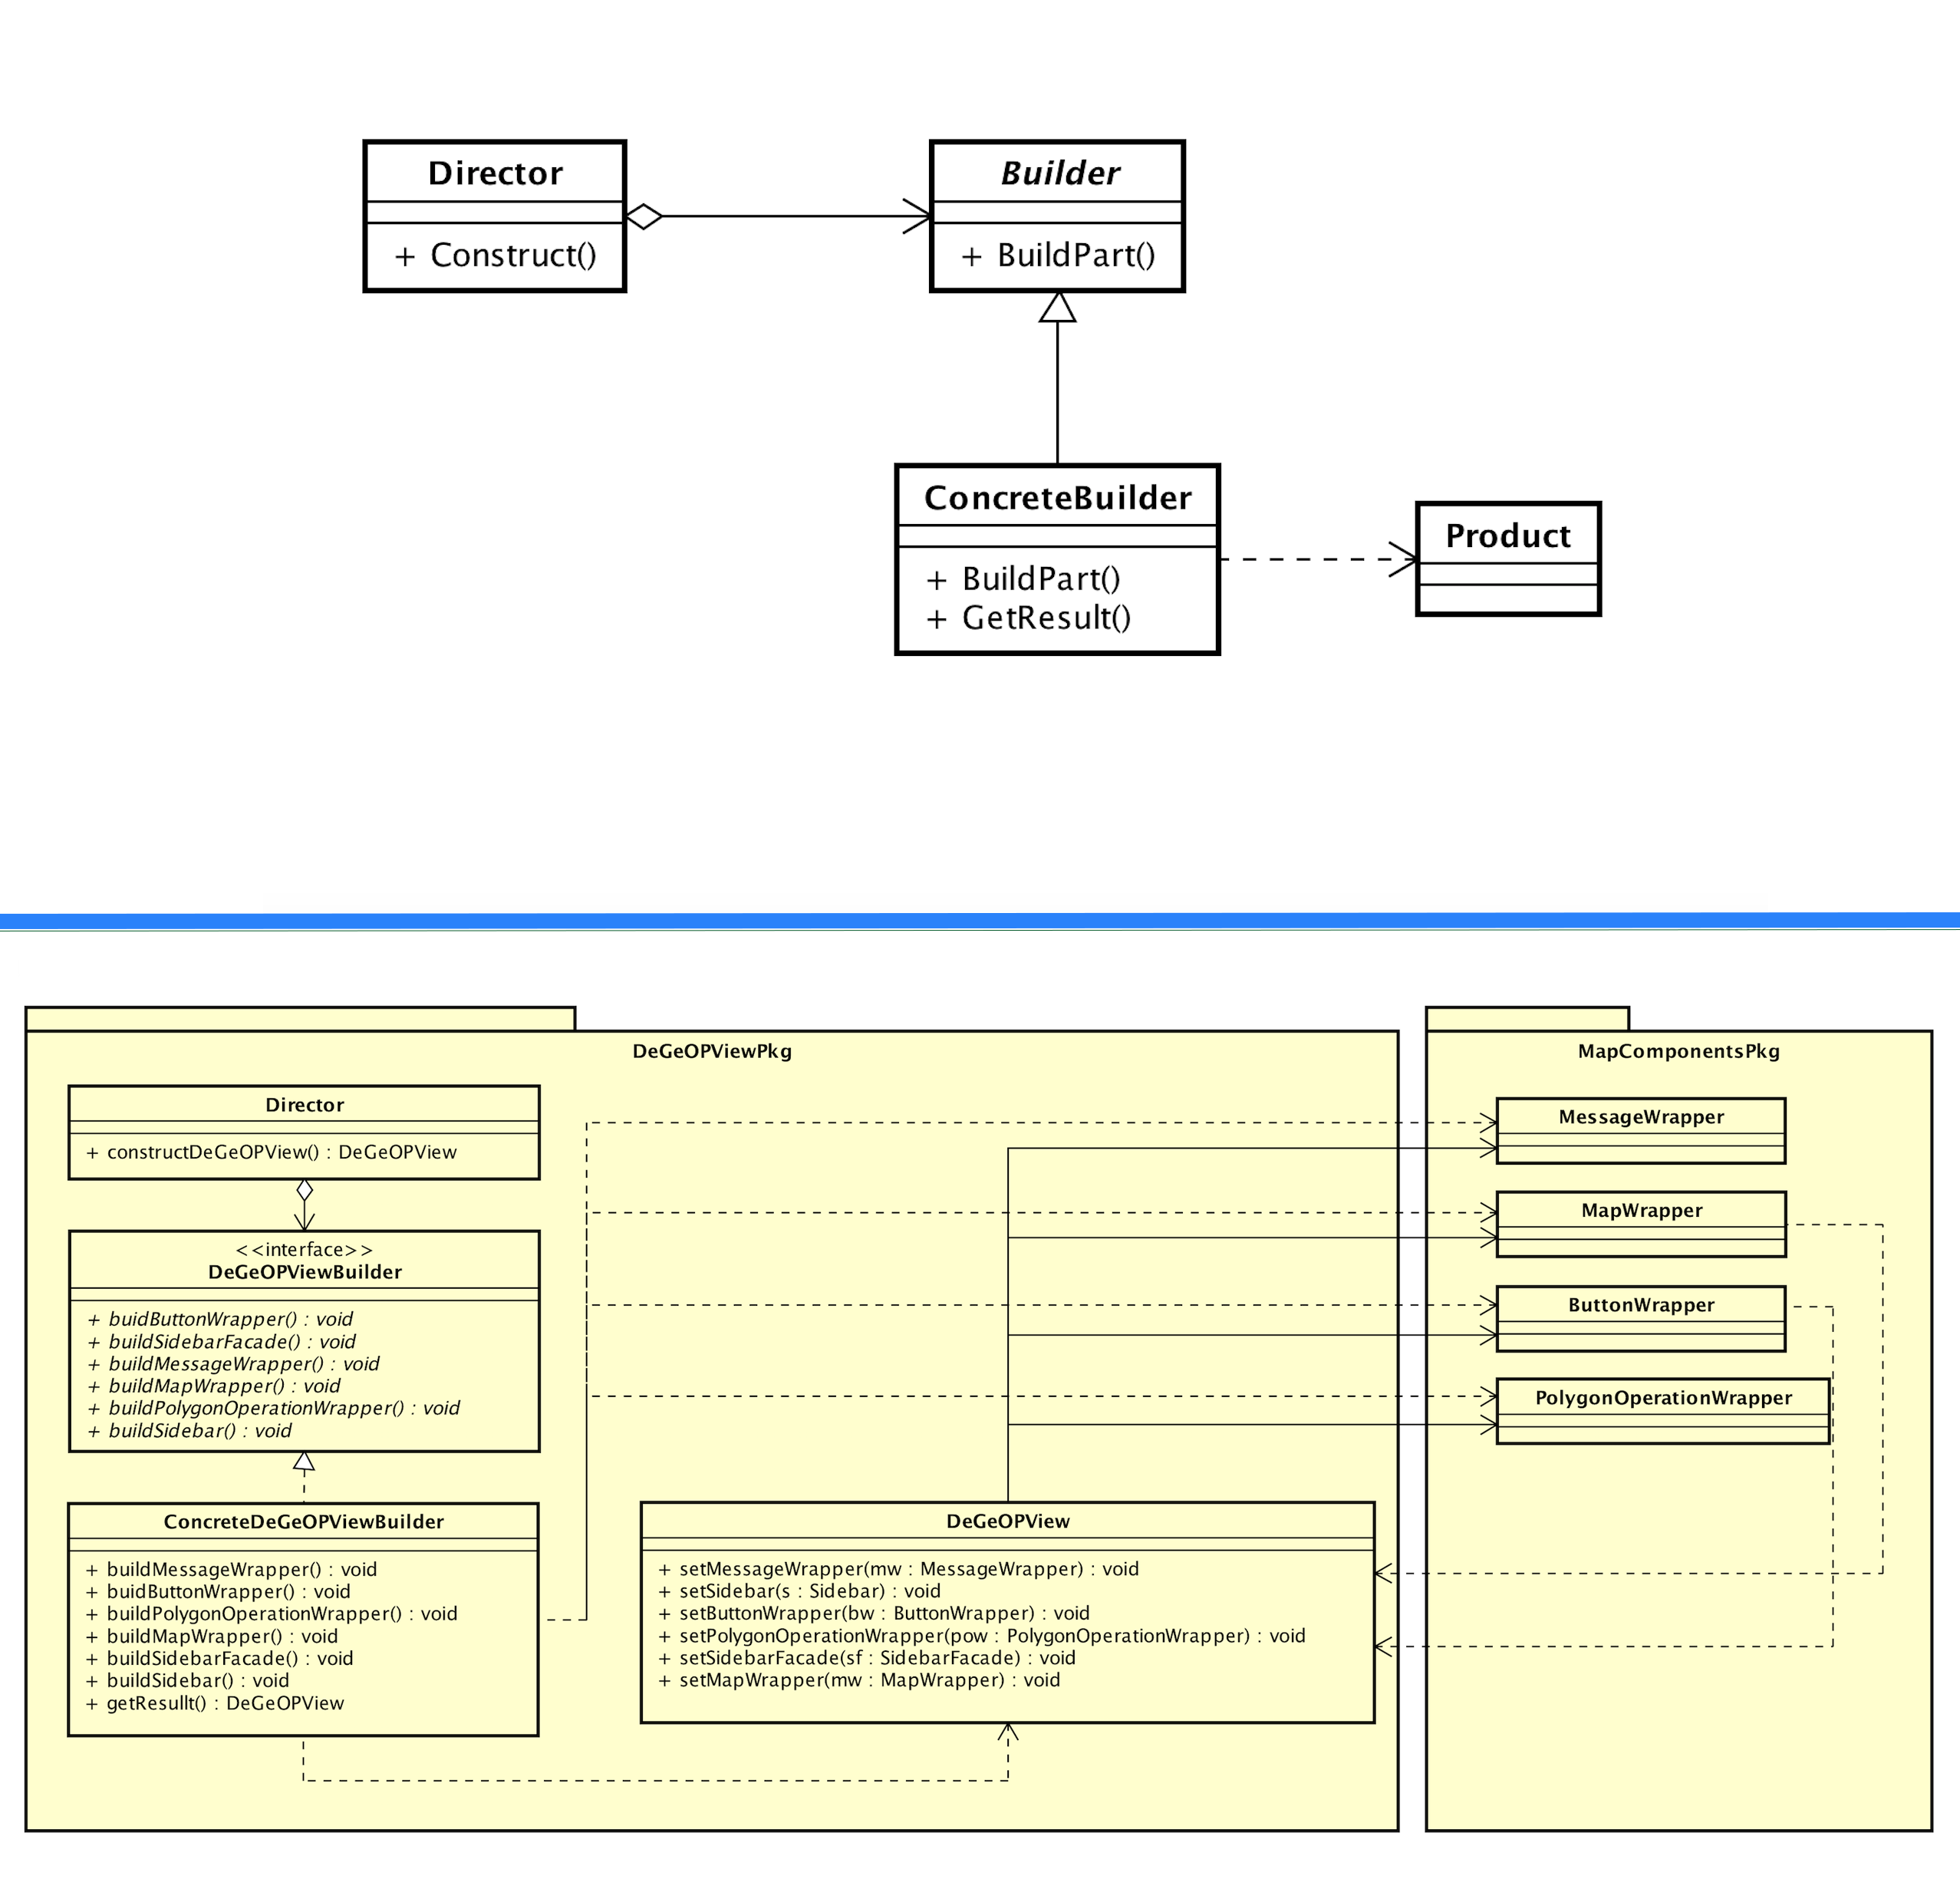
\includegraphics[scale=0.13]{img/builderComparati.png}
		\caption{Builder e la sua contestualizzazione in \progetto}
	\end{figure}

\newpage
\subsubsection{Factory Method}
\paragraph{Descrizione}
Questo pattern permette di creare oggetti fornendo un'interfaccia per creare un oggetto, ma lascia che le sottoclassi decidano quale oggetto istanziare.
Il pattern factory può essere utilizzato quando:
\begin{itemize}
\item 
La creazione di un oggetto preclude il suo riuso senza una significativa duplicazione di codice.
\item 
La creazione di un oggetto richiede l'accesso ad informazioni o risorse che non dovrebbero essere contenute nella classe di composizione.
\item
La gestione del \glo{Ciclo di vita}{ciclo di vita} degli oggetti gestiti deve essere centralizzata in modo da assicurare un comportamento coerente all'interno dell'applicazione.
\end{itemize}
\paragraph{Contestualizzazione}
Questo pattern viene utilizzato nel package \texttt{StorePkg::PolygonPkg}. Sono state create le classi \texttt{ConcretePolygon}, che implementa l'interfaccia \texttt{Polygon}, e \texttt{ConcretePolygonFactor}y, che implementa l'interfaccia \texttt{PolygonFactory}. \texttt{PolygonFactory} espone il metodo \texttt{CreatePolygon}, che viene sovrascritto dalla sua sottoclasse \texttt{ConcretePolygonFactory} consentendo quindi ai suoi utilizzatori, \texttt{Scenario} e \texttt{\glo{Asset}{Asset}}, la creazione dell'oggetto di tipo \texttt{Polygon}.
	\begin{figure}[H]
		\label{builder_compara}
		\centering
		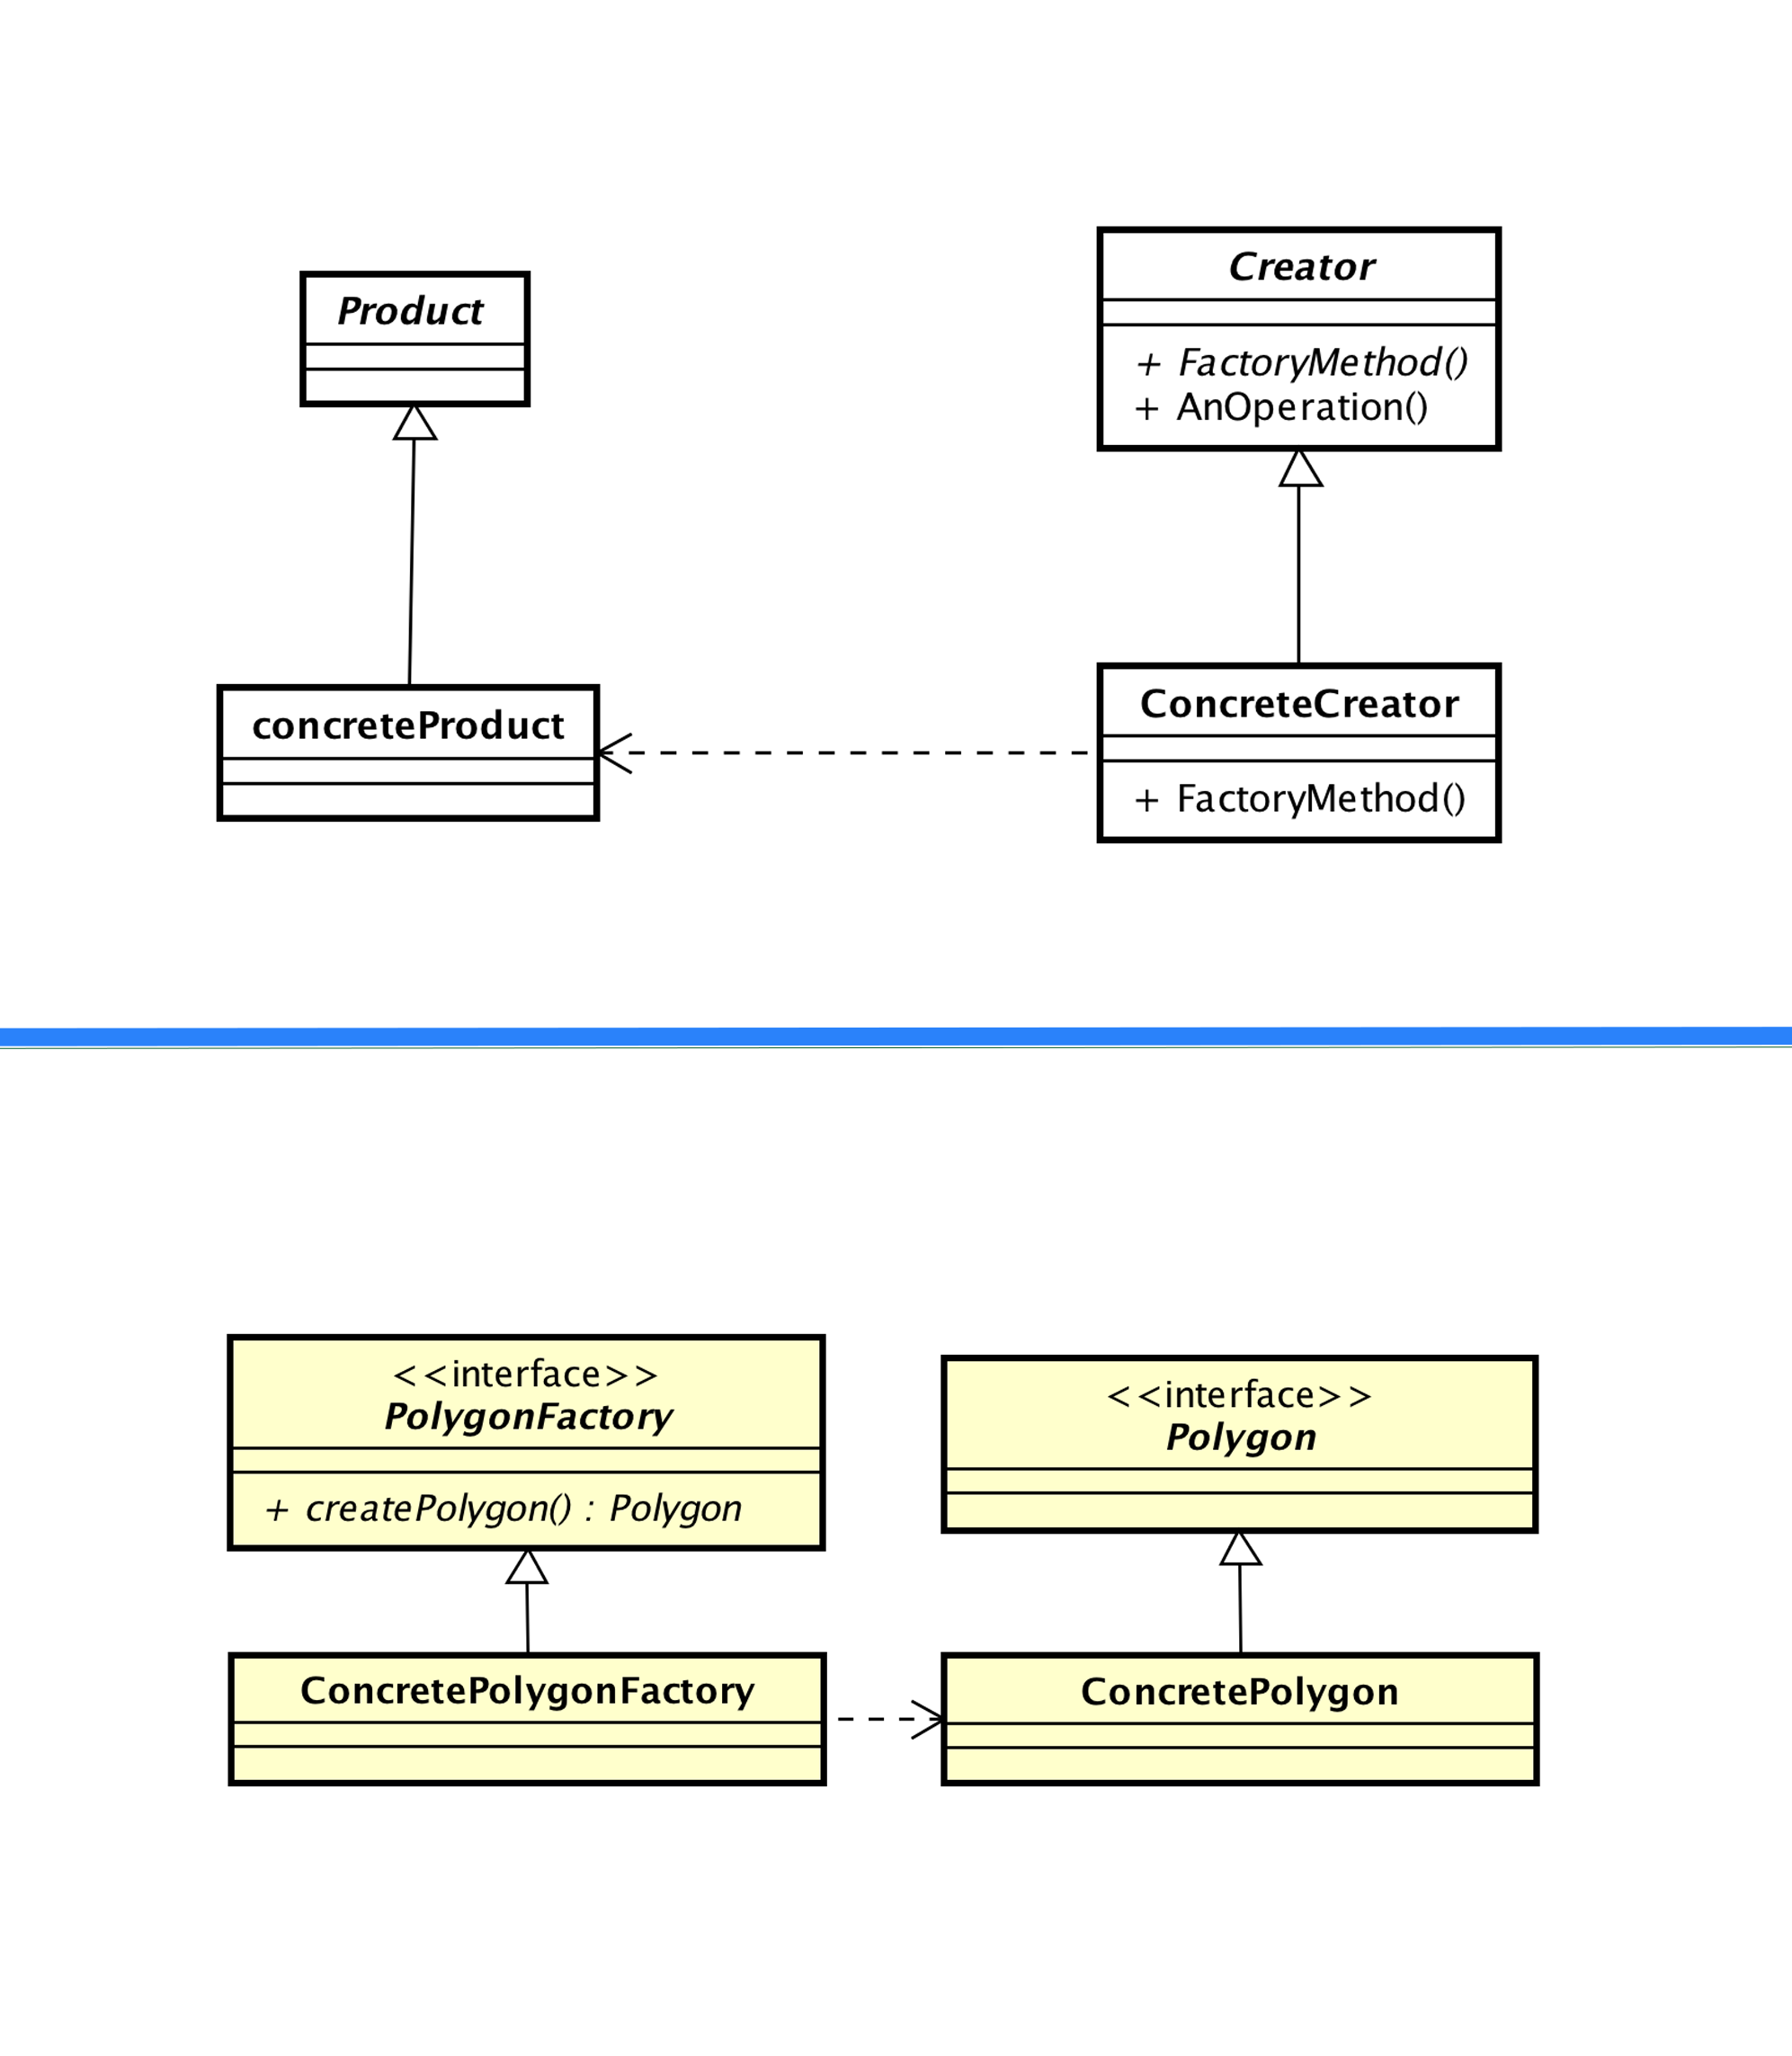
\includegraphics[scale=0.14]{img/factoryComparati.png}
		\caption{Factory Method e la sua contestualizzazione in \progetto}
	\end{figure}


\newpage
\subsubsection{Singleton}
\paragraph{Descrizione}
Il singleton è un design pattern creazionale che ha lo scopo di garantire la creazione di una e una sola istanza di una determinata classe e di fornire un punto di accesso globale a tale istanza.
\\Solitamente questo pattern viene implementato mettendo privato il costruttore della classe interessata e gestendo gli accessi all'oggetto con chiamate statiche per ottenere l'unico riferimento (anch'esso statico) alla classe. La creazione dell'oggetto può avvenire per un metodo di inizializzazione o la prima volta che si tenta di accedere all'istanza di classe.
\\Il Singleton pattern viene comunemente usato nell'implementazione di abstract Factory e Builder e a volte nell'implementazione di Facade od oggetti stato.
	\begin{figure}[H]
		\label{builder_compara}
		\centering
		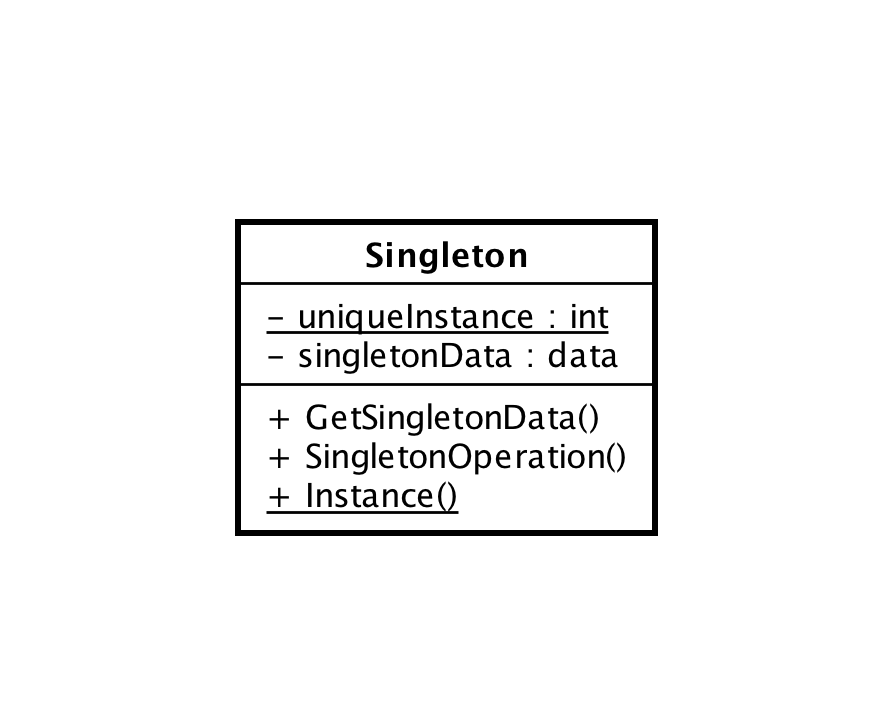
\includegraphics[scale=0.7]{img/singleton.png}
		\caption{Diagramma del Singleton}
	\end{figure}
	
\paragraph{Contestualizzazione}
Molte classi dell'applicazione sono singleton per costruzione.
Viene riportato l'elenco delle classi singleton (il percorso è da considerarsi relativo a partire da DeGeOP::).
\begin{itemize}
	\item StorePkg::AnalysisPkg::AnalysisContainer;
	\item StorePkg::CustomerContentsPkg::Customer;
	\item StorePkg::PolygonPkg::PolygonFactory;
	\item StorePkg::PolygonPkg::ConcretePolygonFactory;
	\item ReducerPkg::Reducer;
	\item ReducerPkg::AssetReducer;
	\item ReducerPkg::NodeReducer;
	\item ReducerPkg::EdgeReducer;
	\item ReducerPkg::ScenarioReducer;
	\item ReducerPkg::AnalysisReducer;
	\item ActionCreatorPkg::AssetActionCreator;
	\item ActionCreatorPkg::NodoActionCreator;
	\item ActionCreatorPkg::EdgeActionCreator;
	\item ActionCreatorPkg::ScenarioActionCreator;
	\item ActionCreatorPkg::AnalysisActionCreator;
	\item CallManagerPkg::CallManager;
	\item CallManagerPkg::DataFromServer;
	\item CallManagerPkg::DataToServer;
	\item View::Director;
	\item View::DeGeOPViewBuilder;
	\item View::ConcreteDeGeOPView;
	\item View::MapPkg::DeGeOPView;
	\item View::MapPkg::MessageWrapper;
	\item View::MapPkg::MapWrapper;
	\item View::MapPkg::ButtonWrapper;
	\item View::MapPkg::PolygonOperationWrapper;
	\item tutte le classi contenute in View::SidebarPkg.
\end{itemize}

\newpage
\subsection{Pattern Strutturali}
\subsubsection{Facade}
\paragraph{Descrizione}
Questo design pattern ha lo scopo di fornire un'interfaccia unificata per un insieme di interfacce presenti in un sottosistema. Facade definisce un'interfaccia di livello più alto che rende il sottosistema più semplice da utilizzare.
\paragraph{Contestualizzazione}
Questo pattern viene utilizzato nel package \texttt{ViewPkg}. E' stata creata la classe \texttt{SidebarFacade}, in modo che il client \texttt{DeGeOPView} possa creare le varie tipologie di Sidebar senza la necessità di conoscere le implementazioni dell'interfaccia factory.
	\begin{figure}[H]
		\label{builder_compara}
		\centering
		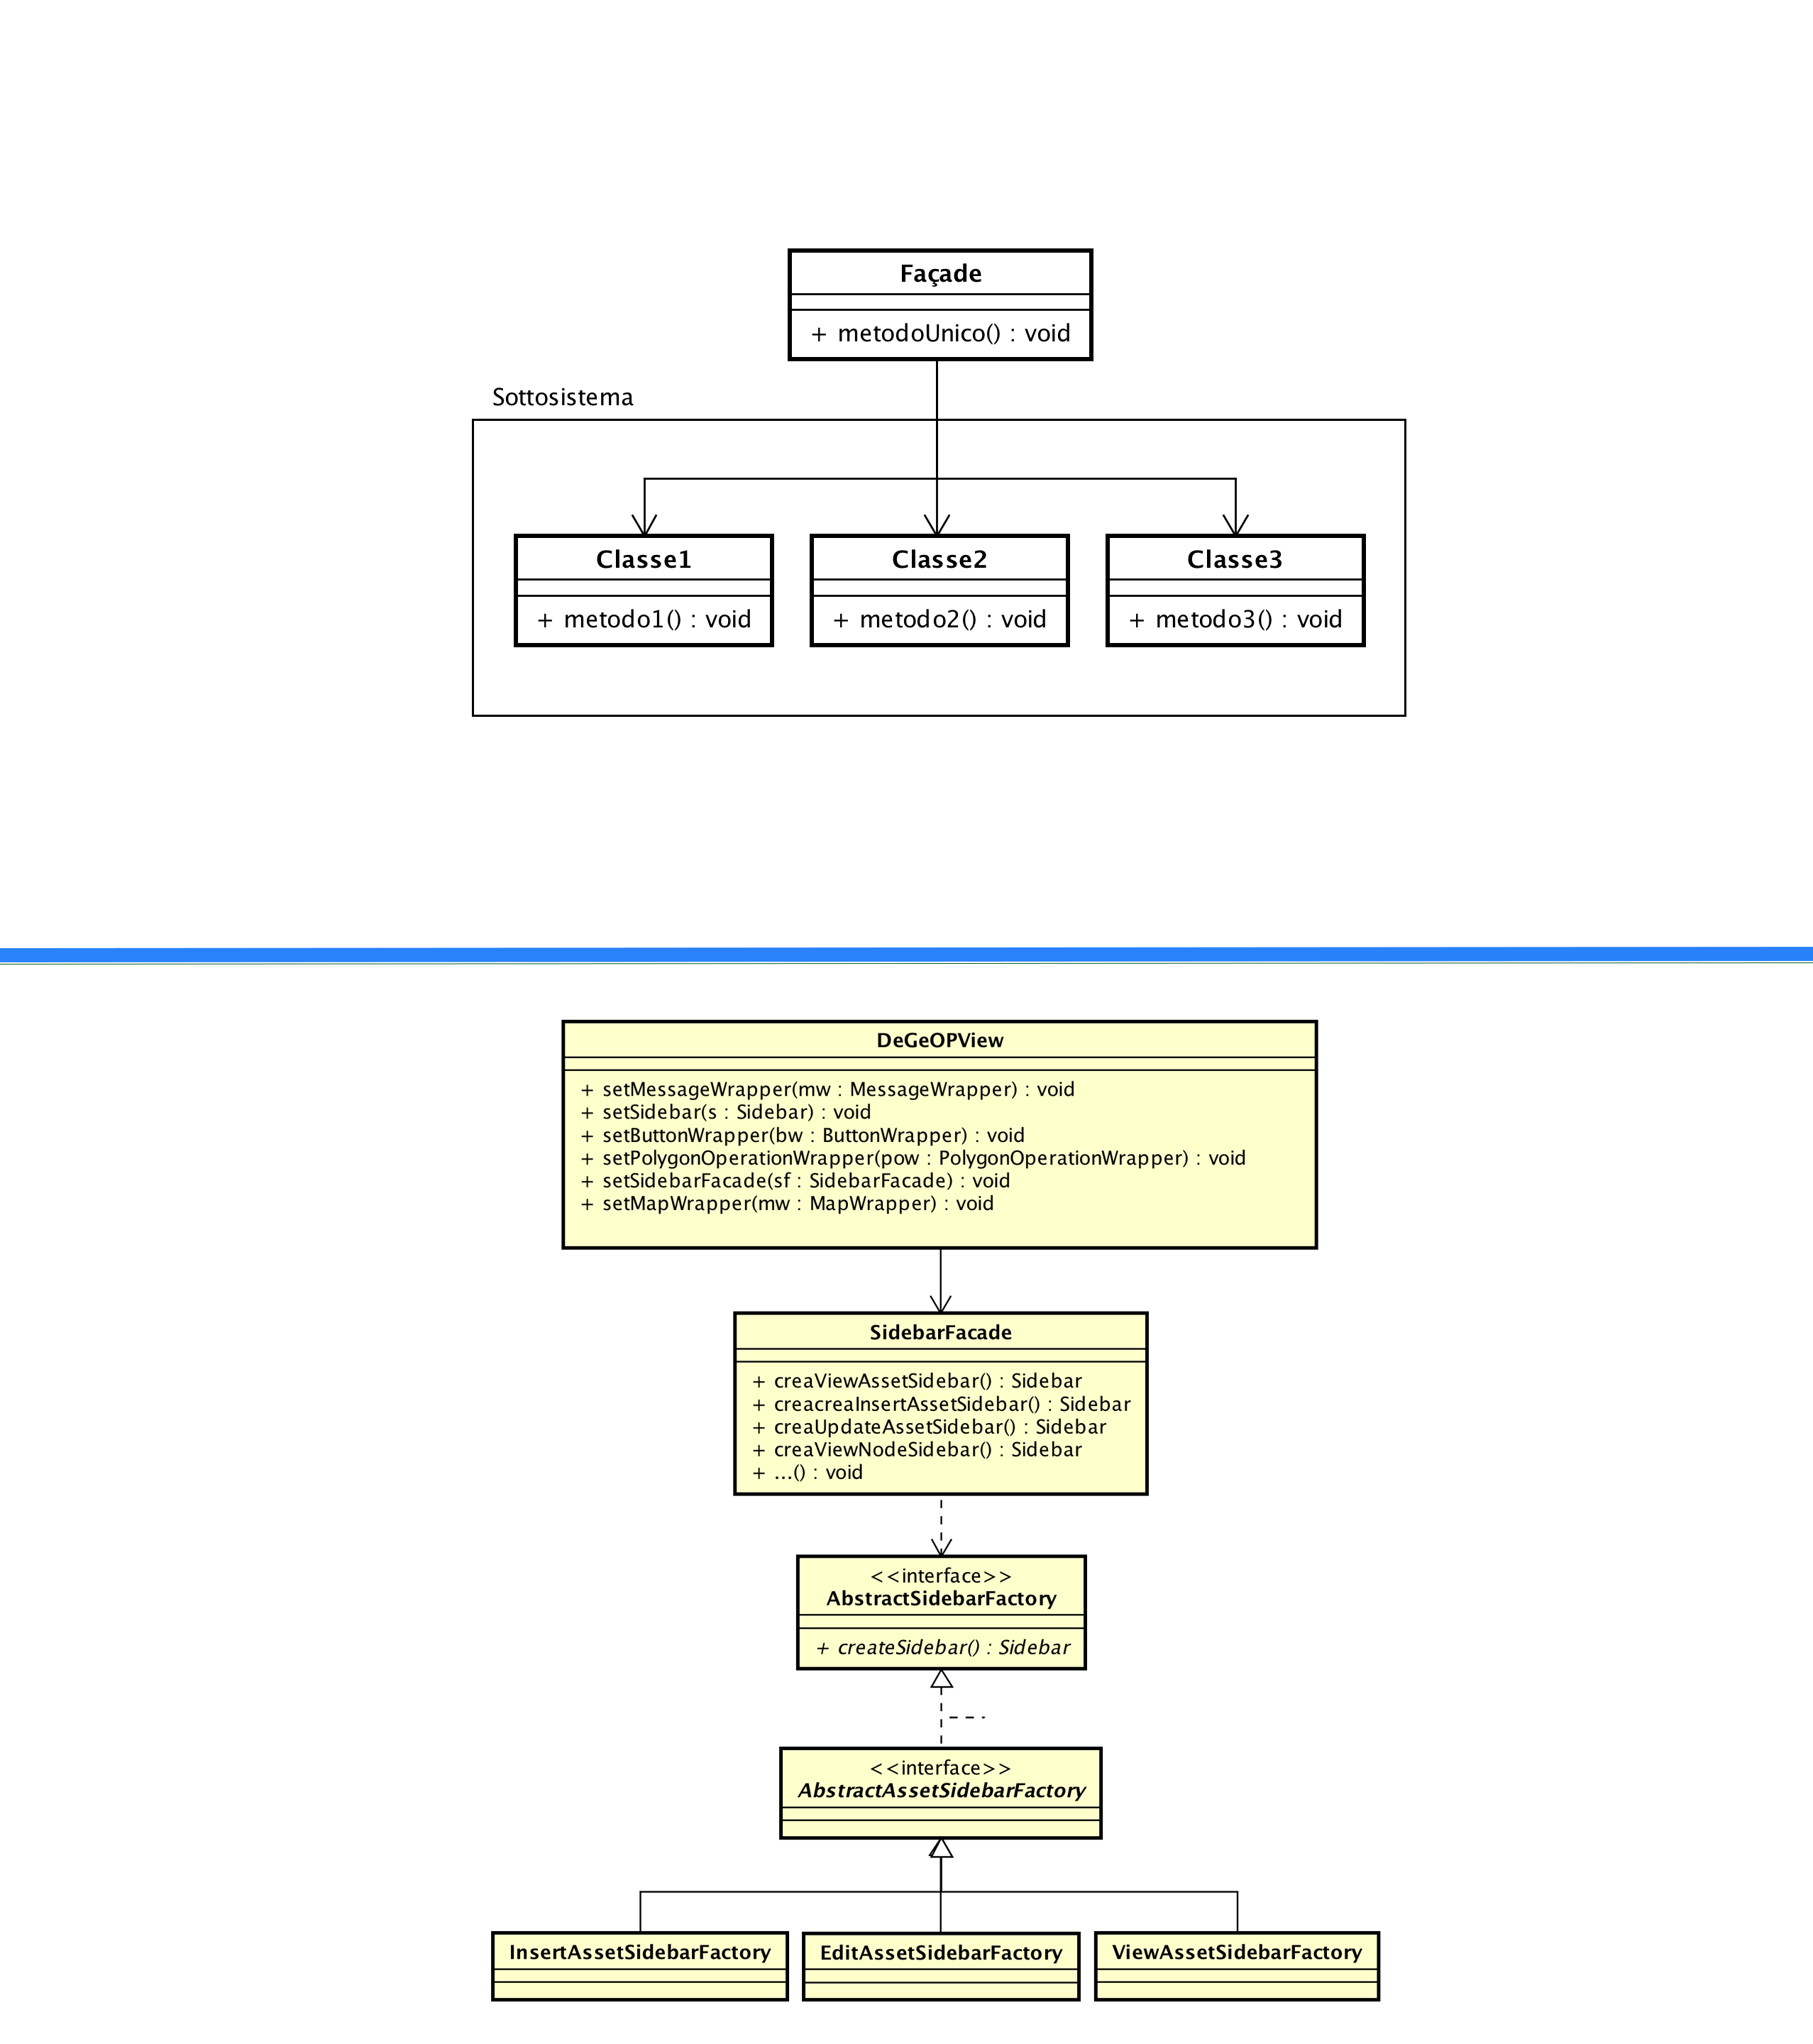
\includegraphics[scale=0.15]{img/facadeComparati.png}
		\caption{Facade ed estratto della sua contestualizzazione in \progetto}
	\end{figure}


\newpage
\subsection{Pattern Architetturali}
\subsubsection{Redux}
\label{dp_redux} % non togliere!
\paragraph{Descrizione}
Il pattern proposto dalla libreria Redux comprende 3 componenti:
\begin{itemize}
	\item \textbf{\glo{Store}{Store}}: è un unico oggetto globale read-only che contiene i dati da gestire, memorizzando l'intero stato del programma;
	\item \textbf{Actions}: definiscono le azioni che si occupano di aggiornare lo Store: l'unico modo di cambiare lo Store è emettere un'azione;
	\item \textbf{\glo{Reducer}{Reducer}}: funzioni pure che, ricevuto un input uno stato e un'azione, restituiscono un nuovo stato modificato in base all'azione.
\end{itemize}
Dato uno Store e una funzione Reducer, lo stato del programma viene aggiornato in modo deterministico con i dati delle azioni.
Il vero punto di forza di Redux è la gestione del flusso di dati in modo unidirezionale. Questo significa che tutti i dati dell'applicazione seguono lo stesso flusso, rendendo la logica dell'applicazione più predicibile e facile da capire e implementare.
\paragraph{Contestualizzazione}
Questo design pattern viene utilizzato per il design dell'architettura ad alto livello, come illustrato nella sezione \nameref{descrizione_architettura} e \nameref{tecnologie}. L'intera applicazione nel suo insieme implementa questo design pattern.
\\Le classi \texttt{\glo{Action}{Action}} all'interno del package \texttt{ActionPkg} e \texttt{Reducer} all'interno di ReducerPkg implementano rispettivamente le componenti Action e Reducer di questo design pattern.
\\L'unico modo per cambiare i dati contenuti all'interno del package \texttt{StorePkg} è emettere delle Actions.
	\begin{figure}[H]
		\label{redux_compara}
		\centering
		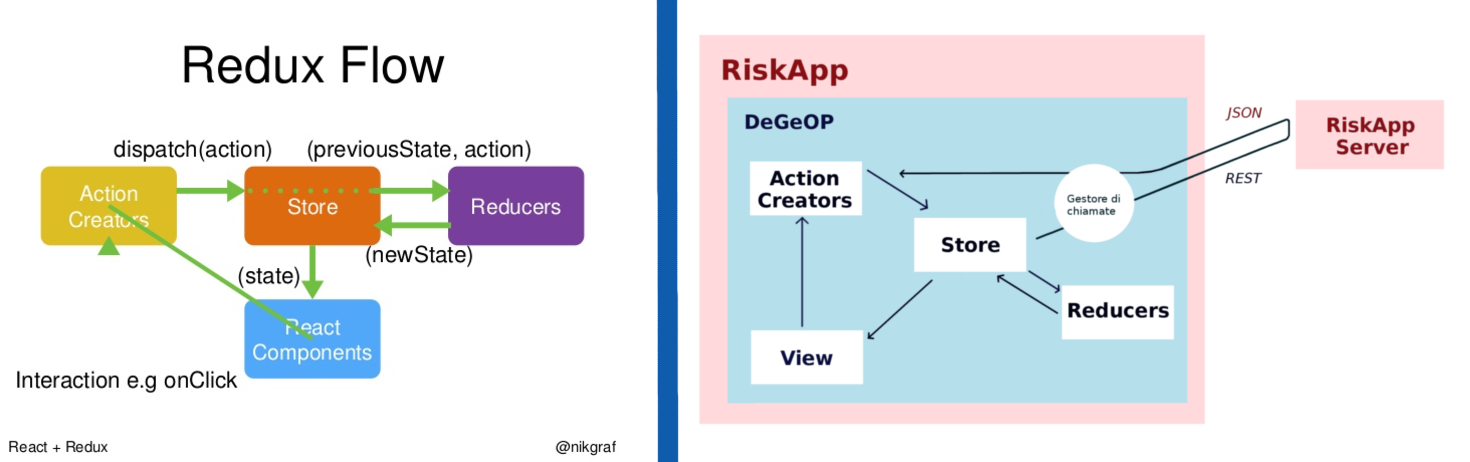
\includegraphics[scale=0.3]{img/ComparaArch.png}
		\caption{Design pattern proposto da Redux e la sua contestualizzazione in \progetto}
	\end{figure}